\documentclass{homework}

\title{Prova 1 - Estrutura de Dados 2020.2}
\author{Carlos Bravo}

\begin{document}

\maketitle

Usando a seguinte definições para os exercícios:
\begin{lstlisting}[language=C]
#define max(a,b) (a>b?a:b)
#define PAI(x) (((x)-1)/2)
#define FESQ(x) (2*(x)+1)
#define FDIR(x) (2*(x)+2)

typedef struct _element{
  int chave;
  struct _element *ant;
  struct _element *prox;
} element;

typedef struct _Node{
  int chave;
  int altura;
  struct _Node *esq;
  struct _Node *dir;
} Node;

typedef struct _Heap{
  int *array;
  int nelem;
  int tam;
}Heap;

Heap *heap;
\end{lstlisting}
\newpage

\exercise
(1.1) Busca em LDECD
\begin{lstlisting}[language=C]
element* busca(element* head, int x){

  element *aux = head->prox; // A partir do primeiro elemento
  
  while(aux != head){ // Enquanto nao chegar no inicio
    if(aux->chave == x) return aux; // Retorna se encontrar
    aux = aux->prox; // Senao continua percorrendo
  
  }
  
  return NULL; // Se chegou aqui nao encontrou
}
\end{lstlisting}
(1.2) Remoção em LDECD
\begin{lstlisting}[language=C]
void remocao(element* head, int x){

  element *aux = head->prox; // A partir do primeiro elemento
  
  while(aux != head && aux->chave != x){
    // Enquanto nao chegar no inicio nem encontrar
    aux = aux->prox; // Percorre
  }
  
  // Se voltou pro inicio, nao encontrou
  if(aux == head) return;
  
  // Atualiza os ponteiros pra pular ele
  aux->ant->prox = aux->prox; 
  aux->prox->ant = aux->ant;
  
  free(aux); // E libera da memoria
}
\end{lstlisting}

\exercise
(2.1) Preencher altura de uma árvore binária
\begin{lstlisting}[language=C]
int getAltura(Node* node){

  //Se eh NULL altura eh 0
  if(node == NULL) return 0;
  
  return node->altura;
}

Node* preencheAltura(Node *node){

  if(node == NULL) return NULL;
  
  // Pra cada no percorre os dois lados
  Node* aux = node;
  aux->esq = preencheAltura(node->esq);
  aux->dir = preencheAltura(node->dir);
  
  // E atualiza a altura
  aux->altura = 1 +
    max(getAltura(aux->esq),getAltura(aux->dir));
  return aux;
}
\end{lstlisting}
(2.2) Inserir elementos em uma árvore binária enquanto atualiza altura
\begin{lstlisting}[language=C]
Node* insere(Node *root, int x){

  // Se eh NULL, insere o elemento
  if(root == NULL){
    root = (Node *)malloc(sizeof(Node));
    root->chave = x;
    root->esq = root->dir = NULL; 
  }else{
    // Se for menor que o atual, vai pra esquerda
    if(x < root->chave){
      root->esq = insere(root->esq,x);
    }else{ // Senao direita
      root->dir = insere(root->dir,x);
    }
  }
  
  // Atualiza a altura
  root->altura = 1 +
    max(getAltura(root->esq),getAltura(root->dir));
  return root;
}
\end{lstlisting}

\exercise
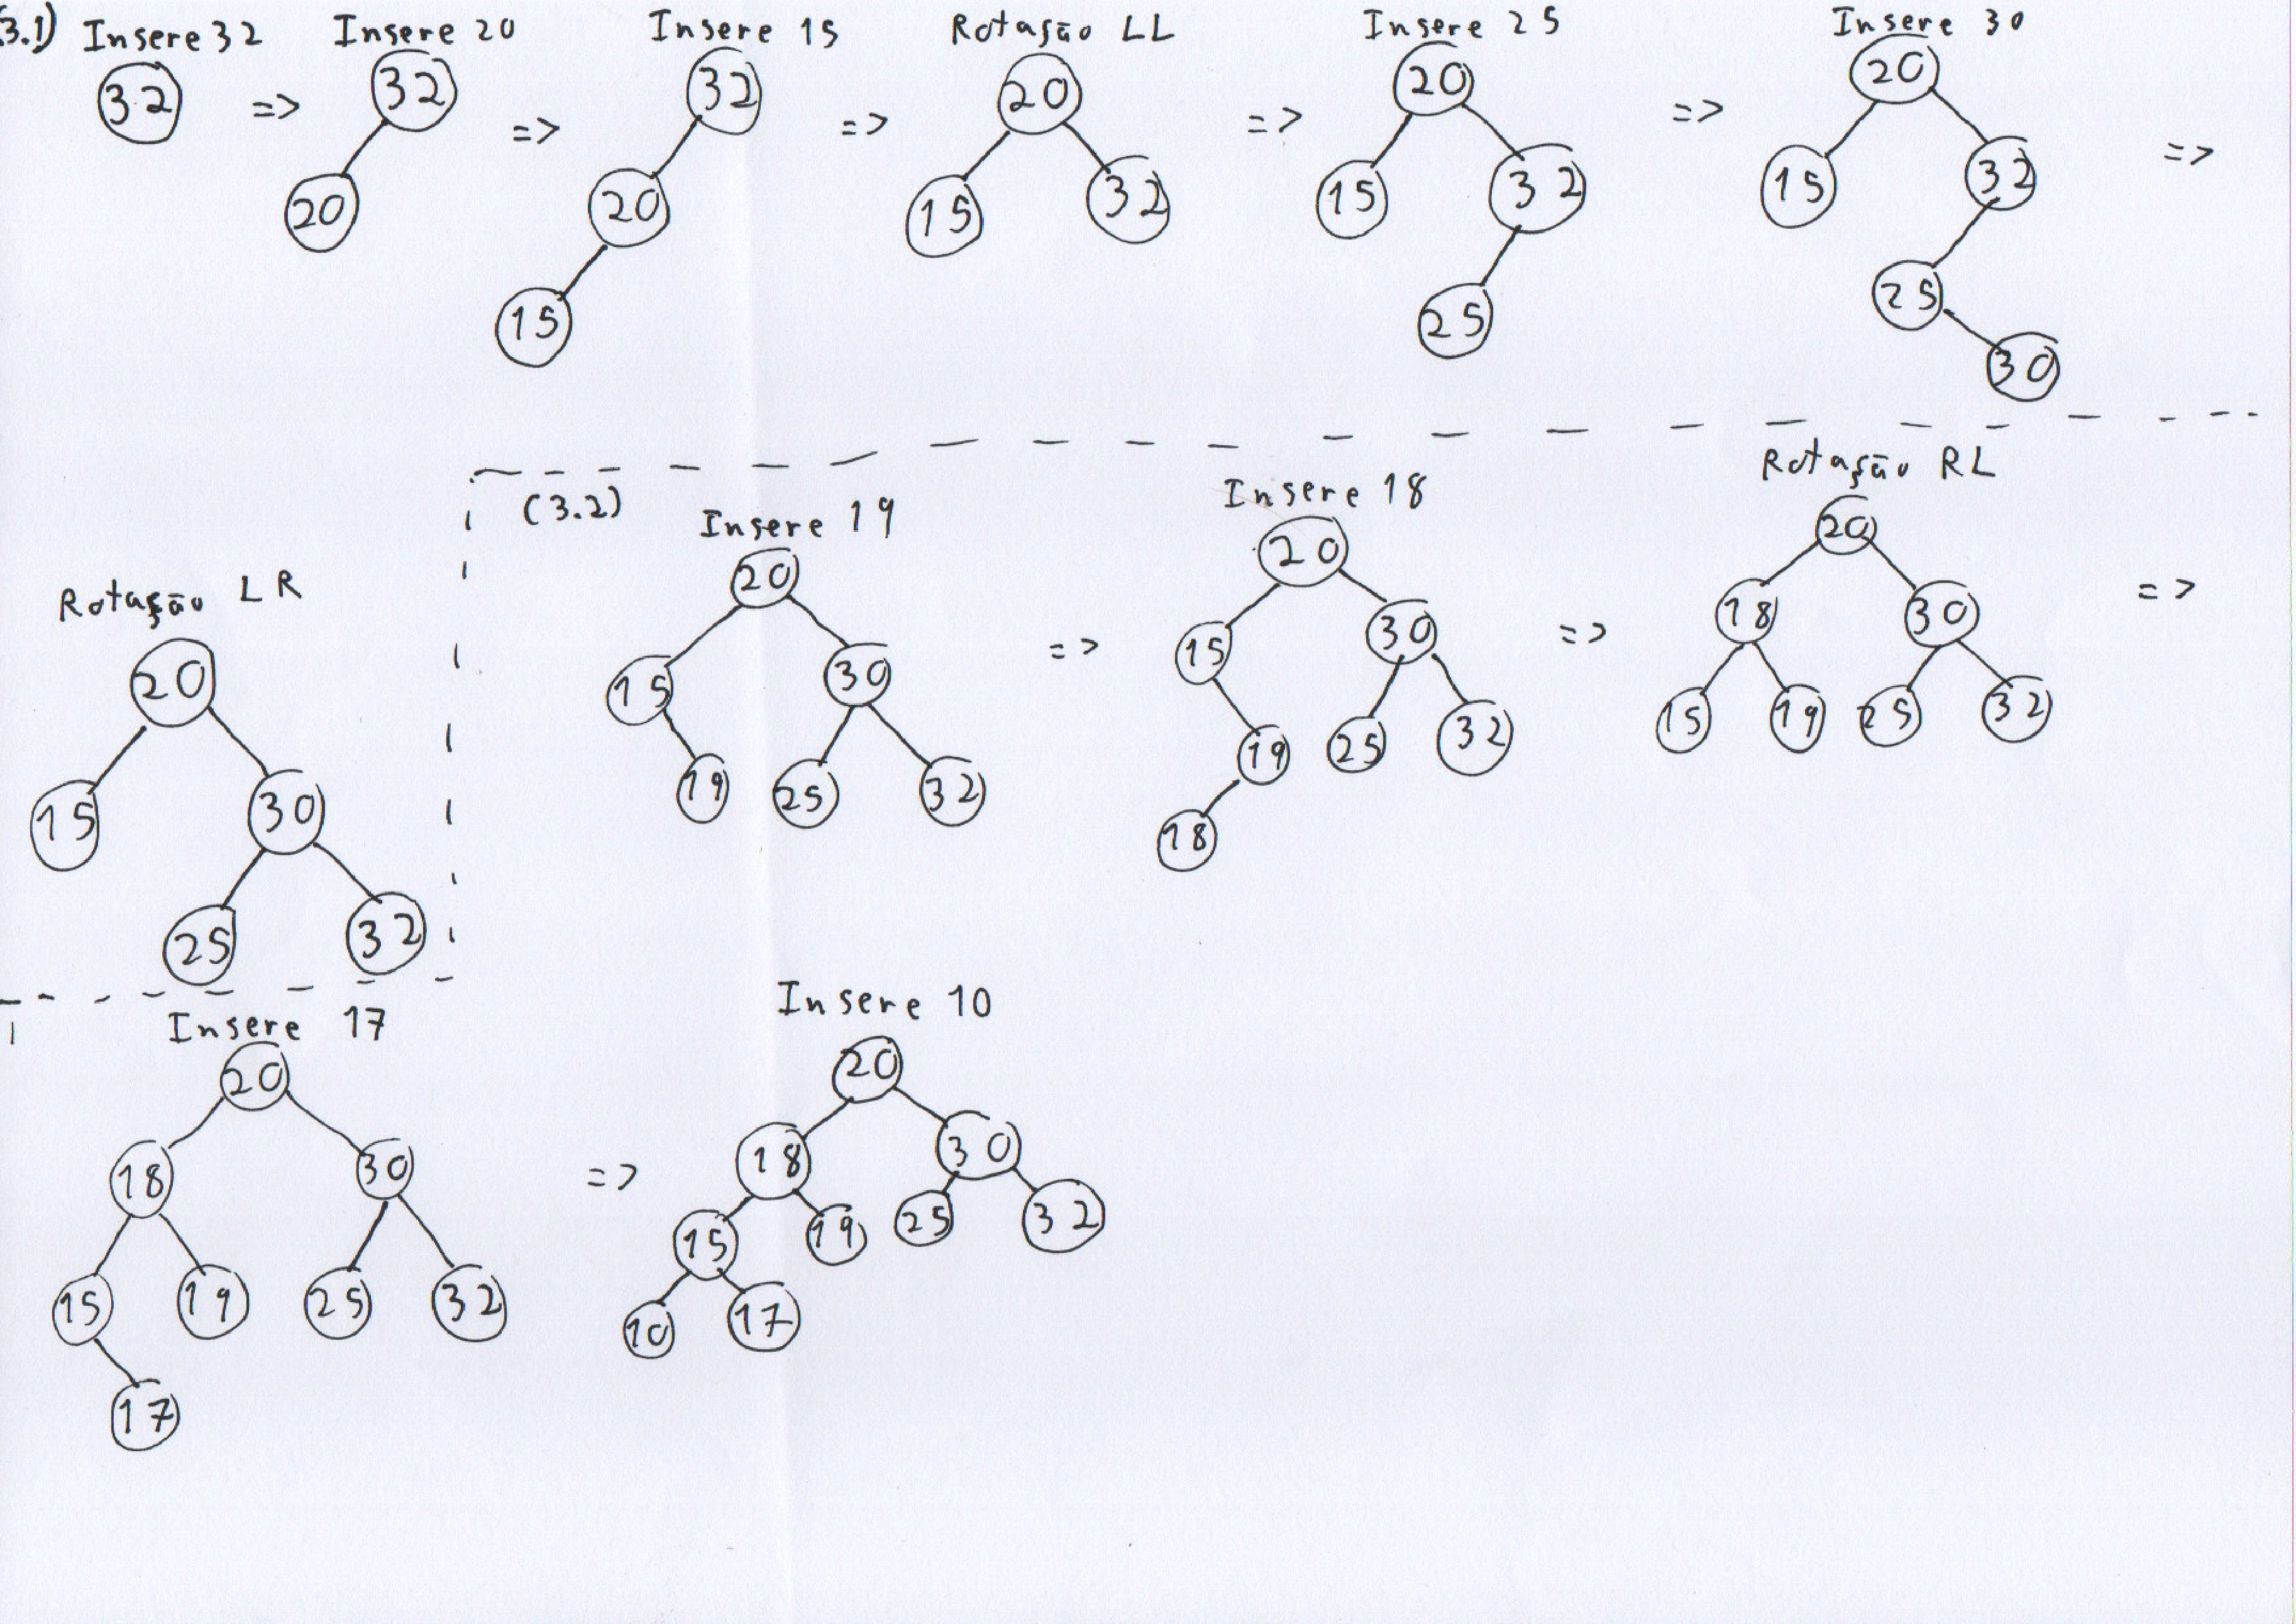
\includegraphics[scale=0.22]{images/q3.pdf}

\exercise*
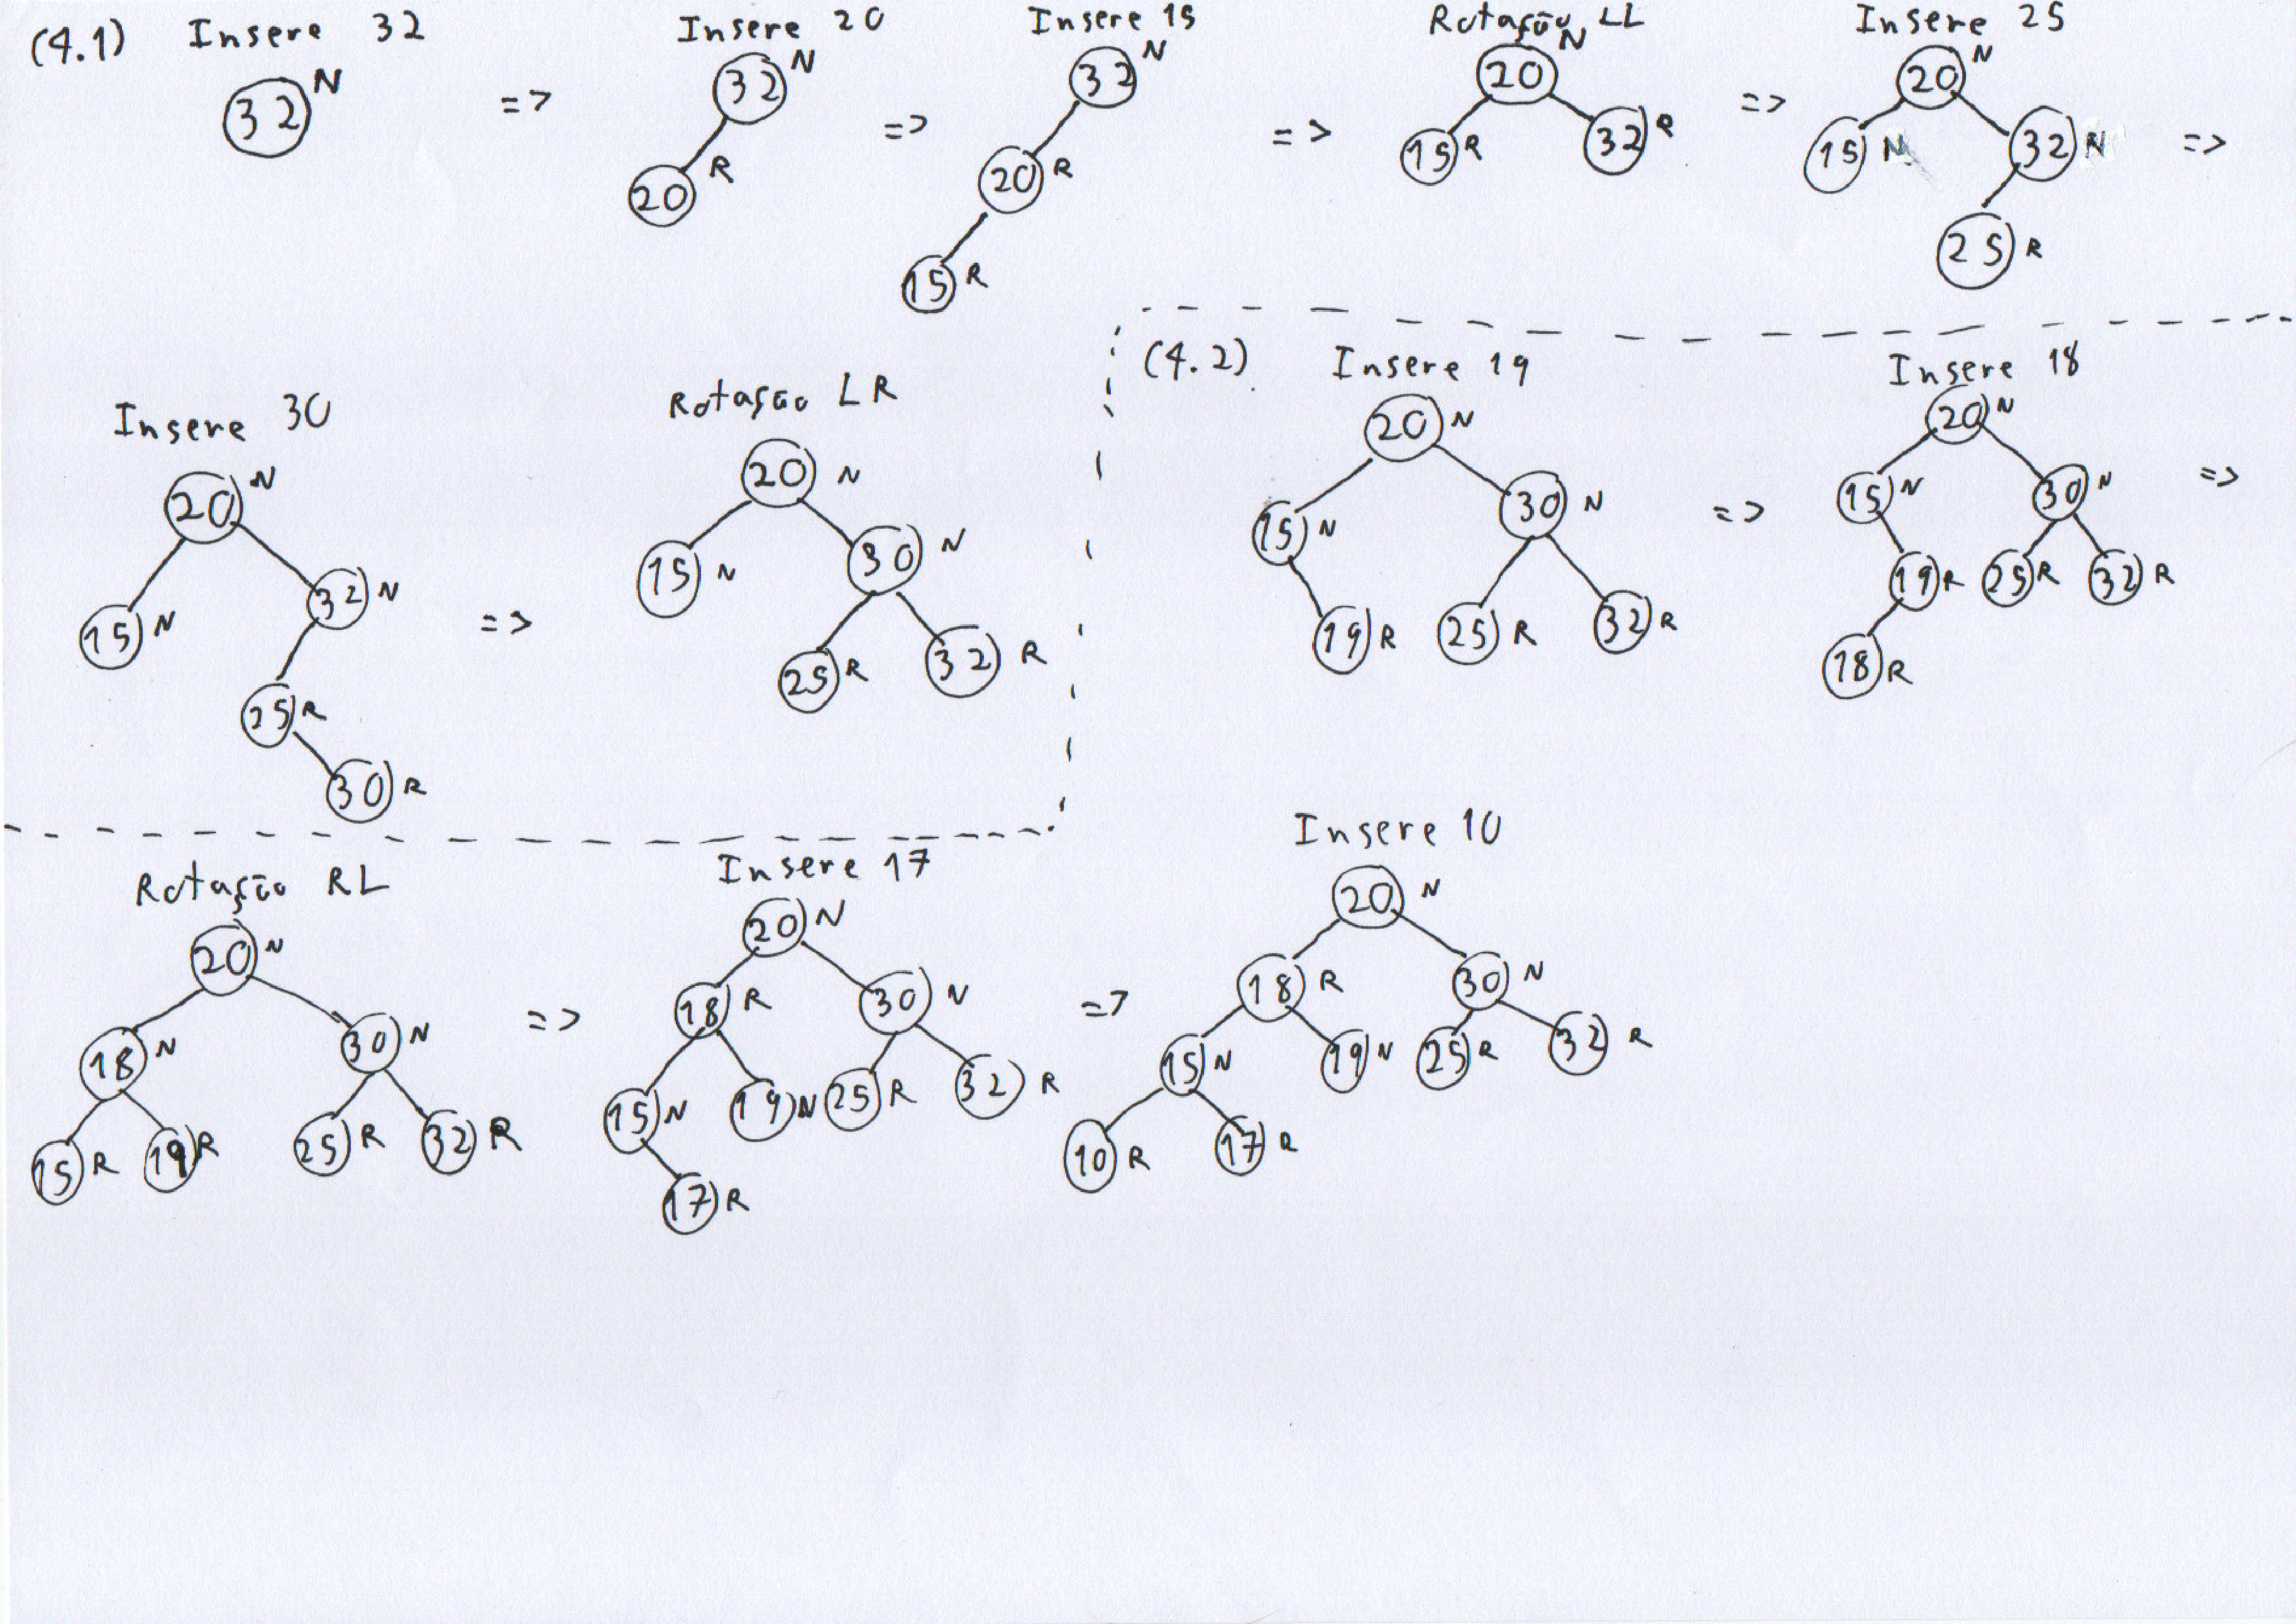
\includegraphics[scale=0.22]{images/q4.pdf}

\exercise
(5.1) Podemos transformar o array em uma heap utilizando o seguinte algoritmo:
\begin{lstlisting}[language=C]
void descer(int pos){
  // Obtem a posicao do filho esq e diz que eh o menor
  int esq = FESQ(pos);
  int menor = esq;
  
  // Se esq nao estiver fora do limite
  if(esq < heap->nelem){
    // Obtem a posicao do filho dir
    int dir = FDIR(pos);
    
    // Se nao estiver fora do limite
    // e for menor que o esquerdo
    if(dir < heap->nelem
      && heap->array[esq] > heap->array[dir]){
        menor = dir; // Atualiza o menor
    }
    
    // Se o atual for maior que o menor filho tem que trocar
    if(heap->array[pos] > heap->array[menor]){
      int t = heap->array[pos];
      heap->array[pos] = heap->array[menor];
      heap->array[menor] = t;
      descer(menor); // Depois de trocar, desce nessa linha
    }
  }
}

void criaHeap(int array[], int nelem){
  // Define a heap e seus parametros
  heap = (Heap *)malloc(sizeof(Heap));
  heap->array = array;
  heap->nelem = nelem;
  heap->tam = 12;
  
  // Para cada no da penultima camada para cima, desce a heap
  for(int i = PAI(nelem-1); i >= 0; i--){
    descer(i);
  }
}
\end{lstlisting}
(5.2) Executando o algoritmo o vetor fica no seguinte formato:
\[
\begin{bmatrix}
5 & 6 & 13 & 8 & 22 & 15
\end{bmatrix}
\]

\newpage
(5.3) Usando o algoritmo de inserção e inserindo na heap o vetor fica no seguinte formato:
\[
\begin{bmatrix}
5 & 6 & 13 & 7 & 18 & 15 & 20 & 8 & 11 & 22
\end{bmatrix}
\]
\begin{lstlisting}[language=C]
void subir(int pos){
  if(pos){ // Enquanto nao estiver na raiz
    int pai = PAI(pos); // Pega a pos do pai
    // Se o pai for maior, troca e sobe nessa linha
    if(heap->array[pai] > heap->array[pos]){ 
      int t = heap->array[pos];
      heap->array[pos] = heap->array[pai];
      heap->array[pai] = t;
      subir(pai);
    }
  }
}

void insere(int x){
  // Se nao tem espaco suficiente, aumenta o tamanho do vetor
  if(heap->nelem == heap->tam){
    overflow();
  }
  // Adiciona o elemento em ultimo lugar e sobe a partir dele
  if(heap->nelem < heap->tam){
    heap->array[heap->nelem] = x;
    subir(heap->nelem);
    heap->nelem++;
  }
}
\end{lstlisting}
\newpage

(5.4) Usando o algoritmo de remoção e removendo a chave mínima o vetor fica no seguinte formato:
\[
\begin{bmatrix}
6 & 7 & 13 & 8 & 18 & 15 & 20 & 22 & 11
\end{bmatrix}
\]
\begin{lstlisting}[language=C]
void removeMin(){

  if(heap->nelem == 0){
    printf("Heap vazia\n");
    return;
  }
  
  heap->nelem--;
  
  // Passa o ultimo elemento pra raiz pra continuar balanceado
  // E desce a partir do primeiro
  heap->array[0] = heap->array[heap->nelem];
  descer(0);
}
\end{lstlisting}

\end{document}
